\newcommand{\CLASSINPUToutersidemargin}{1.5in}
\documentclass[10pt,final,journal]{IEEEtran}
\usepackage{graphicx}

\begin{document}
\title{Scalable Transaction Processing for Cloud Datastores through Optimized Partitioning}
\author{Benjamin Busjaeger, Jonathan Chu, Daniel Ormond \\
\{busjaeg2, jmchu2, ormond1\}@illinois.edu}
\date{Feb 2012}
\maketitle

\begin{abstract}
We are designing a new cloud data storage system that will be highly scalable and yet still be able to provide strong data consistency guarantees. Our system extends existing cloud key/value stores with modular components for transaction management and access-based partitioning. We plan to utilize clustering algorithms from the machine learning field to co-locate related data for efficient transaction processing and to assign partitions to optimal locations in the server clusters. Through continuous analysis of execution logs, our system should be able to recognize data access patterns and use that knowledge to partition data within the cluster to better fit within those patterns. With our data partitioning scheme, we hope to lower time delays, reduce bandwidth, and ultimately improve the speed of online transaction processing without sacrificing data consistency.
\end{abstract}

\begin{IEEEkeywords}
cloud, data storage, transaction processing, partitioning
\end{IEEEkeywords}

\section{Introduction}
As more and more companies begin moving their applications to the cloud, there is a greatly increasing rise in the amount of data that needs to be distributed and managed. As they progress, emerging businesses need to maintain high performance as they scale up to their growing client base. On the Internet, network traffic can be highly volatile and quickly shift from peak loads to low loads as clients attempt to commit transactions and modify their information. As such, websites need to have a robust, distributed database system that can handle a large number of transactions and queries while still guaranteeing consistency of the data. 

Old, relational database designs like mySQL focused on the ACID properties of atomicity, consistency, isolation, durability. However, in the new age of big data, it is now necessary to use multiple nodes and servers to run enterprise level applications. MySQL databases are not built to scale with multiple nodes which makes them too slow with heavy data intensive traffic. The CAP theorem states that it is impossible to have all three of consistency, availability, and partition tolerance at the same time. However, databases can still have two of the three, and new noSQL databases were created to emphasize the BASE properties in contrast to the ACID properties of mySQL. These BASE properties focused instead on availability and relaxed the consistency constraint. In this paper, we are developing a mechanism to draw models of relationships from data to enhance these BASE properties for certain unique situations where data may have a relationship with other parts of the database, but still want to run on a noSQL datastore. These NoSQL datastores distribute data across many nodes to scale horizontally and thus ensure fast parallel performance in serving customers.

One such scenario could involve storing documents for a company where business spreadsheets might need to be pulled, updated, removed, or added. A business may have a diverse range of datasets and documents to use in their day to day operation and may have thousands of employees who need access to the data. This would be a scenario that involves a heavy amount of data that needs to be highly available for business transactions and could benefit from the properties of a noSQL datastore. A document store like that would have implicit relationships between certain documents and should be arranged in a datacenter to better reflect those relationships. At the same time, the property of consistency could be relaxed so that documents could be highly available for modification by employees. In this case, a document may have only a few owners that could possibly access it and data may rarely have conflicts. That is why companies should strive to achieve the quickest possible transaction times while still maintaining eventual data consistency.

The move to distribute databases creates new challenges in the form of data partitioning and placement. It is difficult for a programmer to manually partition databases and to see the relationships between data. He may be required to analyze complex data access patterns and understand the implications on database performance. Furthermore, manual partitioning puts a burden on the programmer that instead could be handled by software to improve application and development time. By delegating partitioning to the storage system, application developers can spend their time elsewhere in the development of their websites. Finally, there may be certain web applications which have a complex structure and chain of data accesses that may not be feasible for a human to efficiently analyze.

To provide scalable performance, an effective data partitioning scheme is needed which co-locates related data and assigns partitions to nodes such that bandwidth consumption is minimized and response time reduced. We propose to develop a transactional datastore along with a new methodology for partitioning data that utilizes machine learning. By using machine learning algorithms to train on past data access patterns, we believe we can create a new approach for data partitioning that will be more effective than those developed in the past.

In response to the lack of scalability and high operational cost of traditional RDBMSs, large Internet companies have developed their own data storage solutions. The most notable examples include Google's BigTable ~\cite{Chang:2006:BDS:1267308.1267323}, Yahoo's PNUTS ~\cite{Cooper:2008:PYH:1454159.1454167}, and Amazon's Dynamo ~\cite{DeCandia:2007:DAH:1323293.1294281}. These key/value databases automate many aspects of distributed storage, but provide limited consistency guarantees and lack partitioning schemes optimized for transaction processing.

\section{Related Work}
Research on large-scale OLTP systems appears to be coming from at least two directions. On one hand, numerous approaches have been proposed recently for extending BigTable-like datastores with more powerful transaction models. On the other hand, several recent publications describe how to adapt RDBMSs to make them more suitable for cloud workloads. The common theme across these approaches is a departure from full featured ACID transactions across the full data set. The proposals either reduce transaction isolation levels to make global transactions feasible or restrict serializable transactions to a subset of the data. In the latter case selection of these subsets is critical for ensuring efficient transaction processing, so algorithms have emerged to automate this process. We will first examine and classify OLTP cloud datastore architectures and subsequently survey relevant work on optimized data partitioning.

\subsection{OLTP Cloud Datastores}
\emph{Cloud SQL Server} ~\cite{Campbell:2010:ESF:1807167.1807280, Bernstein:2011:AMS:2004686.2005651}, \emph{ElasTraS} ~\cite{Das:2009:EET:1855533.1855540, Das:2010:EAE}, and \emph{Relational Cloud} ~\cite{Curino:2011:JPMWMBZ11} describe approaches for scaling out different relational DBMSs. Cloud SQL Server augments Microsoft SQL Server with partitioning and primary-copy replication. Serializable ACID transactions are supported, but limited to a single partition. A partition can be a whole logical database, referred to as a table group, if it is sufficiently small, or a set of rows from a table group that have been assigned a common partitioning key by the user in the database schema. ElasTraS uses hierarchical schema-level partitioning and also restricts transactions to one partition. It differs from Cloud SQL Server in that it decouples storage from metadata management through the use of a distributed file system. This allows for a dynamic mapping between partitions and nodes. Relational Cloud combines a workload-aware approach for efficient data placement with a graph-based partitioning algorithm for data co-location discussed in the next section. ACID transactions are supported within and across partitions. Although our approach is not targeted at RDBMSs, it shares some of the partitioning ideas.

\emph{Percolator} ~\cite{Peng:2010:LIP:1924943.1924961}, \emph{HBaseSI} ~\cite{Zhang:2010:5697970} and \emph{ReTSO} ~\cite{Junqueira:2011:LTS:2056318.2057148} are different approaches for adding global transactions with snapshot isolation semantics to BigTable-like datastores. Percolator is specifically designed to allow incremental search index construction, so it is optimized for throughput and not suitable for latency-sensitive applications. HBaseSI is a pure client API that uses a set of custom tables and atomic test-and-set operations to manage transactions without central coordination. ReTSO implements a lock-free commit algorithm using a centralized Transaction Status Oracle. Our approach provides a stronger form of isolation and is neither fully decentralized nor centralized. Nevertheless, it builds on several ideas from these publications to implement a non-invasive and efficient concurrency control protocol.

\emph{G-Store} ~\cite{Das:2010:GSD:1807128.1807157} and \emph{CloudTPS} ~\cite{Wei:2011:5740834} build transaction capabilities targeted at specific use cases on top of BigTable-like datastores. G-Store introduces a key group protocol to provide ACID transactions over a dynamically selected set of keys. It is intended for applications which need to execute transaction across frequently changing groups of entities, that are non-overlapping, so it has limited applicability. CloudTPS is designed for web application workloads and assumes short-lived transactions that access small data sets known prior to starting the transaction. It interposes a group of Local Transaction Managers (LTMs) between clients and datastores which load data items and transaction state into memory for efficient processing. This implies the need for a separate server cluster with its own fail-over and recovery mechanisms.

\emph{Deuteronomy} ~\cite{Levandoski:2011:8530161} defines a transaction component (TC) capable of providing full ACID transactions for any datastore that implements a well-defined data component (DC) interface. The TC applies concurrency control and undo/redo logging at the logical record level as opposed to at the physical page level. Our transaction manager also operates against an abstract datastore contract to make it portable. However, it uses different concurrency control and recovery algorithms and does not rely on a centralized TC.

\emph{MegaStore} ~\cite{Furman:2008:8530095, Baker:2011:8530095} tries to bridge the gap between RDBMSs and NoSQL datastores by providing strong consistency guarantees within fine-grained partitions of data and high availability through synchronous cross-data center replication. It also adds a declarative schema language, secondary indices, queues, and distributed transactions on top of BigTable. Our transaction manager is similar to the one used in Megastore in that it relies on multiversion concurrency control and partitioning, but also differs in several ways. First, we implement a concurrency protocol that allows reading uncommitted values, whereas Megastore supports only last committed, snapshot, or inconsistent reads. In Megastore updates are written to a replicated log and then applied to the datastore post commit. Reads within the same logical partition block until changes are applied, whereas reads across partitions may not see committed data. We write mutations directly into the datastore, but filter the result set of read operations. Finally, our transaction manager is scoped to physical partitions, which allows commit optimization across all rows in the partition, whereas Megastore scopes transaction managers to finer grained logical partitions, which makes wide-area network log replication feasible.

\begin{table}[!t]
\renewcommand{\arraystretch}{1.3}
\caption{OLTP Cloud Data Store Classification}
\label{classification}
\centering
\begin{tabular}{|c|c|c|c|}
\hline
\bfseries Data Store  & \bfseries Data Model & \bfseries  Part. & \bfseries Isolation \\
\hline
\hline
Cloud SQL & relational & yes & serializable \\
ElasTraS & relational & yes & serializable \\
Rel. Cloud & relational & yes & serializable \\
Megastore & BigTable & yes & serializable \\
G-Store & BigTable & yes & serializable \\
CloudTPS & BigTable & no & serializable \\
Deuteronomy & agnostic & no &serializable \\
Percolator & BigTable & no & snapshot \\
HBaseSI & BigTable & no & snapshot \\
ReTSO & BigTable & no & snapshot \\
\hline
\end{tabular}
\end{table}

\subsection{Paritioning Algorithms}
There are multiple partitioning algorithms in use and in study currently.  Not all of the algorithms have the same goal.  Hash-based algorithms help scale the database by evenly distributing the data on different nodes while other algorithms have a more specific goal to reduce transaction overhead.

Schism ~\cite{Curino:2010:SWA:1920841.1920853} is a static partitioning algorithm to reduce distributed transactions for SQL datastores. It uses transaction logs to determine how to partition data. The transaction anaylsis is similar to the work done by Chun-Hung et al.~\cite{chun:2002} It significantly improves performance compared to hash-based and even manual partitioning techniques. These static algorithms are a good starting point for our work and would likely yield better results for key/value stores given their simplified data access model. Also, an incremental version of these algorithms may scale better than the static equivalent, since it may be able to consider only new transaction log entries in each iteration. Another option would be to use a probabilistic algorithm.

Hehme and Bruno ~\cite{Nehme:2011:APD:1989323.1989444} present and algorithm that deeply integrates directly with the parallel query optimizer in Microsoft SQL Server.  Their algorithm provides a static data partitioning recommendation.  Their goals was to provide a data partition strategy in less time than other less deeply integrated solutions.


\section{Background}

\subsection{BigTable}
BigTable ~\cite{Chang:2006:BDS:1267308.1267323} is a distributed storage system for managing structured data. It was developed at Google out of the need to store vast amounts of data (petabytes) across a large number of machines (1000s) with high scalability, availability, and performance. BigTable offers a simple data model that resembles a multidimensional map in which values are indexed by a triple consisting of row key, column key, and timestamp. The map is sparse in that it only persists cells that actually contain data, and it is sorted in lexicographical order by row key. It is also automatically partitioned into row ranges, called \emph{tablets}, which are distributed across machines.

Reads or writes that access data in a single row are atomic and transactions across such operations are also supported. However, transactions that span multiple rows are not supported. Apart from single row operations, the API also includes scanners that can be used to iterate and filter data and a server-side scripting language, called Sawzall ~\cite{Pike:2005}, for more complex read-only queries.

BigTable stores data and logs in the Google File System (GFS) ~\cite{Ghemawat:2003:GFS:1165389.945450}. GFS is a distributed file system optimized for large-scale data-intensive applications. Data is automatically replicated across multiple data nodes and error detection is built-in through checksums. BigTable also relies on Chubby ~\cite{Burrows:2006}, a distributed lock service and file system built on the Paxos algorithm ~\cite{Lamport:1998:PP:279227.279229, Lamport:2001:PMS}, for master election, address boostrapping, and server discovery.

A BigTable cluster consists of clients, a single master, and many tablet servers. The master maintains the set of active tablet servers discovered via Chubby and assigns tablets to tablet servers. Schema manipulation is also handled by the master. Each tablet server manages a set of tablets and responds to read and write requests for those tablets. Each tablet contains the values for all columns and timestamps for each row in the given range of a table. However, since tablets are assigned to balance the load across tablet servers, they are not necessarily co-located with other tablets of the same table. Clients talk directly to tablet servers to access data. To find out which tablet stores the desired rows and where the tablet is currently located, clients query a special metadata tablet whose location is stored in Chubby. As tablets grow or shrink, they are split or merged and moved between servers. The former operation is initiated by tablet servers whereas the latter are initiated by the master.

Tablets are physically stored in GFS as a set of SSTables, which is a file format that implements an ordered immutable map in the form of indexed blocks. Since SSTables are immutable, tablet mutations are first written to a redo log stored in GFS and then added to an in-memory data structure called \emph{memtable}. When the memtable exceeds a certain threshold, a \emph{minor compaction} is triggered, which writes the memtable into a new SSTable. To reduce the number of SSTables, \emph{merging compactions} combine several SSTables into a single one and \emph{major compactions} combine all SSTables into a single one and also permantenly apply delete mutations.

BigTable also implements several refinements to improve performance. Relevant in this context are commit log and tablet recovery optimizations. All redo log records for tablets on a given tablet server are stored in a single log file to reduce disk seeks and enable group commit. The implication is that if a tablet server crashes, the log has to split across tablet servers that are assigned to recover the tablets. Recovery consists of replaying any mutations that have not be stored in SSTables into the new memstore. To avoid this overhead when moving tablets between servers, the source server compacts the tablet once before and once after closing it.

Finally, BigTable was recently enhanced with Coprocessors which allow executing code directly on tablet servers similar to stored procedures in traditional database systems ~\cite{Dean:2009}. Coprocessors are attached to tablets and share their lifecycle. They expose a higher-level call interface than RPC in that clients address row ranges which the client library resolves into actual locations and Coprocessor invocations.

\subsection{HBase}
HBase is an open source implementation of Google's BigTable. For the most part it closely implements the BigTable design, but there are some notable differences ~\cite{George:2011} some of which are relevant in this context. First, HBase uses a different naming scheme. Tablets are referred to as \emph{regions}, memtables are called \emph{MemStores}, and SSTables are called HFiles. Secondly, HBase builds on open source alternatives to GFS and Chubby, namely the Hadoop Distributed File System (HDFS) and Zookeeper ~\cite{Hunt:2010:ZWC:1855840.1855851}.
Thirdly, HBase's coprocessor framework differs slightly from the one used in BigTable. HBase coprocessors are implemented as Java classes that are dynamically loaded by region servers as needed. They fall into two categories: \emph{observers} or \emph{endpoints}. Observers are invoked when certain events occur, similar to triggers in traditional database systems. They can be attached to a region, the master, or the write-ahead log to perform additional processing or intercept invocations. Endpoints expose custom operations to execute directly on the server hosting the data.
Our system is built on HBase, so we will use HBase terminology in the following discussion.

\subsection{Multiversion Timestamp Ordering}
Multiversion timestamp ordering (MVTO) is a multiversion concurrency control (MVCC) protocol that generates serializable transaction schedules. It assigns each transaction a unique timestamp that is larger than that of any transaction started before it. It then maps the operations onto versions such that the result is equivalent to that of a serial schedule on version-less data in which transactions are executed in the order of their timestamps. Operations are scheduled optimistically, so if an ordering conflict occurs that cannot be resolved, one of the transactions must be aborted and restarted.

The concrete protocol consists of the following three rules ~\cite{Weikum:2001:TIS}:
\begin{enumerate}
\item A read operation of some object $x$ by transaction $t_i$ is transformed into a read operation of the latest version of $x$ written by a transaction started before $t_i$.
\item A write operation of some object $x$ is rejected and $t_i$ aborted if a transaction that started after $t_i$ has already read a version of $x$ written by a transaction that started before $t_i$. Otherwise, it is transformed into a write operation of version $i$ on object $x$.
\item A commit operation by transaction \emph{i} is delayed until all transactions that have written versions of objects read by \emph{i} have been committed.
\end{enumerate}

MVTO allows for a higher degree of concurrency than lock-based protocols, because reads can be served from older versions while newer ones are being created. It is also deadlock free, since no locks are used and transactions only ever wait on transactions started before them to commit. In addition, recovery is simplified, because data is never modified in place. To undo a write means to simply remove the written version. It should also be pointed out that MVTO prevents the write skew anomaly permitted by snapshot isolation protocols as illustrated in figure ~\ref{si}. The first transaction is forced to abort when it attempts to write a new version of \emph{y} by rule two, since the second transaction has already read the previous version. These advantages come at the cost of potential transaction retries and additional storage overhead for temporary versions.

\begin{figure}[!t]
\centering
\hspace*{-.2in}
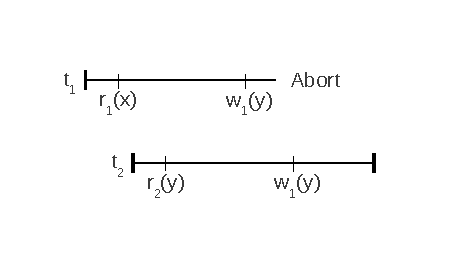
\includegraphics{images/si.pdf}
\caption{Write skew prevention}
\label{si}
\end{figure}

\section{Transaction Manager}
To provide extended transaction management capabilities, we augment HBase with three components: a timestamp oracle (TSO), a region transaction manager (RTM), and a transaction client (TC). The TSO is a centralized server whose sole purpose is to generate globally unique and monotonically increasing timestamps. The RTM is a special coprocessor responsible for managing transactions for all operations that access rows in its associated region. Although it is optimized for local transactions, it is also capable of partiticpating in transactions that span several RTMs. The TC wraps the HBase client to augment the HBase API with transaction interfaces. It interacts with the TSO to obtain new timestamps and with the RTMs to manage transactions. It should be noted that this design does not require a centralized coordinator or any changes to HBase itself. Figure ~\ref{tm} shows these components side-by-side with the HBase components. Zookeeper is the underlying fabric used by all components except by the TSO, so it is not shown in the diagram. The following subsections discuss these components in detail.

\begin{figure}[!t]
\centering
\hspace*{-.15in}
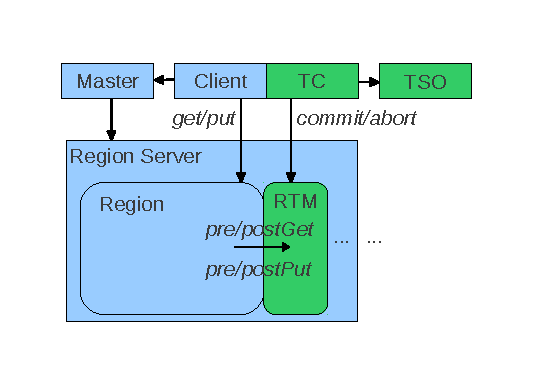
\includegraphics{images/tm.pdf}
\caption{Transaction Manager}
\label{tm}
\end{figure}

\subsection{Region Transaction Manager}
The RTM implements full ACID transactions for operations accessing any row in a single region. It does this by intercepting all read and write operations through the region observer coprocessor interface. It also exposes a coprocessor endpoint through which TCs issue local commit and abort operations. One RTM instance is associated with each region in the cluster.

At the core of the RTM is a recoverable implementation of the MVTO concurrency control protocol. The properties of MVTO make it particularly well suited for implementing transactions on top of BigTable datastores. Timestamps are already built into the data model, so they can be used to store transaction timestamps. The immutable nature of MVTO is in line with one of the core design principles underlying BigTable, namely exploiting immutability to avoid synchronization and to leverage garbage collection. Finally, BigTable is designed to dynamically scale as data grows, so it can more easily cope with the additional storage overhead for temporary versions than centralized database systems. Although our MVTO implementation is applied to HBase regions, it is designed to be datastore agnostic, so any datastore that satisfies the constraint model can be used with it.

\subsubsection{Writes}
The RTM is notified by the region whenever a row is about to be written and immediately after it was written. It processes the before-write notification by applying the second rule of the MVTO protocol for each column in the row touched by the write: If an older version of any column in the row has already been read by a younger transaction, then the current transaction is aborted. The RTM also remembers each cell written by the transaction so that it can remove them in case the transaction is aborted. Although the write itself is executed as an atomic unit, the notifications are not part of that unit. In particular, it is possible for a read operation to occur in between a write and one of the corresponding notifications. Therefore, the RTM also remembers which writes are currently in progress until it receives a notification indicating that they have completed.

\subsubsection{Reads}
Read operations retrieve all versions in the row whose timestamps are smaller than that of the transaction. The result set is passed to the RTM as part of the post-read notification, so it can filter it based on the first rule of the MVTO protocol. For each column in the row it traverses the versions in descending order and applies the following algorithm: if the current version was written by an aborted transaction, the version is removed from the result set and the next is tried. Otherwise, the RTM records that the transaction read this version and removes all older versions of this column from the result set. If the transaction that wrote the version is still active, the RTM also records a read-from relationship between the transactions, so it can delay the commit or cascade aborts as needed. Prior to iterating over the versions, the RTM also checks if a pending write for a newer version exists that should be part of the result set, but is not (because it has not been applied to the region yet). If this is the case, the reading or writing transaction must abort, because the reader has a view of the data that is inconsistent with the timestamp ordering. In other words, the read appears to have been scheduled before the write, however, if that were the case, the write would not have been admitted.

\subsubsection{Deletes}
Deletes are handled as a special case of writes. Clients issue a write operation of a null value annotated with a special delete marker. When the RTM is notified about the write, it remembers this marker, so it can filter deleted cells out read result sets. After the transaction has committed, versions marked as deleted are permanently removed from the region, so they no longer need to be filtered out on reads.

\subsubsection{Aborts and Commits}
When a transaction is aborted, the RTM no longer considers it for write conflict detection. After the abort has been recorded, the RTM asynchronously finalizes the transaction by aborting any transactions that read from it and deleting any versions it has written into the datastore, including delete markers. When a transaction commits, the RTM waits until all transactions it read from have committed before recording the commit. In the asynchronous commit finalizer it notifies transactions that read from the committed transaction about the commit and permanently applies deletes by removing delete markers and all older versions of the given cell in the datastore.

\subsubsection{Version Cleanup}
The operations described above only remove versions from the datastore that were written by aborted transactions or by delete operations of committed transactions. It is also necessary to remove committed versions that have been superseded by newer committed versions. While it would be possible to issue delete operations to the datastore as part of the post-commit finalizers, a more efficient approach is to hook a garbage collector into the region compaction process to simply omit old versions when new HFiles are written. This approach was developed in ~\cite{Junqueira:2011:LTS:2056318.2057148}. For this purpose, RTMs expose an operation that returns the oldest active transaction timestamp at any given time. For each cell, the garbage collector can omit any versions that carry timestamps smaller than that one, except for the last.

\subsubsection{Data Structures}
Each transaction is represented by an in-memory data structure that stores the state, the keys for read and written versions, and references to other transactions it read from. Three separate indices on these transactions are maintained in order to provide for efficient lookup and conflict detection. The main index is a binary search tree on the TID. It is used for direct lookup and to peridiodically scan transactions in the order they started to determine the first active transaction. As part of the scan any finalized aborted transaction is removed from the indices. Any finalized committed transaction that preecedes the first active transaction is also removed and garbage collected. Finalized committed transactions that started after the first active transaction must be kept around, since they may still be needed for conflict detection. The second index stores transactions by versions read and the third by keys they are in the process of writing. These indices make conflict detection for a given key an $O(n \: log(m))$ operations where $n$ is the number of versions for the key and $m$ is the maximum number of transactions that read a given version. Note that version cleanup effectively makes $n$ a constant.

\subsubsection{Recovery}
RTMs must be able to survive region restarts, crashes, splits, and moves. Therefore, the data structures need to be recoverable from persistent storage. RTMs do this by logging each transaction operation to a write-ahead log, which is stored in a table by region. Old log entries are prediodically purged from the table based on the first active transaction timestamp. This reduces resource usage and speeds up the recovery process. When an RTM recovers from a region crash, it replays all log entries into the data structures and then aborts transactions that were active at the time of the crash. Logging could be optimized using group commits ~\cite{Weikum:2001:TIS} on a per-region basis, but we leave this for future work.

\subsubsection{Distributed Transactions}
Although the main goal of this work is to provide means to localize transactions, we also need to support distributed transactions so that applications can initially run unoptimized and our learning algorithm can detect groupings. Users may also have a need for distributed transactions in production in certain situations where grouping is not possible. Distributed transactions are implemented via Zookeeper. When a TC detects the need for a distributed transaction, it creates a special transaction node in Zookeeper that identifies the transaction. Each RTM when asked to enlist in the distributed transaction creates an ephemeral sequence node under the transaction node. The RTM uses the node to vote for the outcome and the TC uses the node to detect server failure and to decide the outcome.

\subsection{Timestamp Oracle}
Globally unique timestamps are needed to ensure that the MVTO protocol generates globally serializable schedules. It would be possible to implement Lamport clocks ~\cite{Lamport:1978:TCO:359545.359563} for this purpose, but using a centralized timestamp server is an approach adopted by many recent distributed transaction managers that rely on timestamp ordering (e.g., ~\cite{Peng:2010:LIP:1924943.1924961, Wei:2011:5740834}). The TSO must be highly available and recoverable. To achieve this, it can use a similar fail-over mechanism to the HBase master, in which a hot-standby monitors Zookeeper to take over if the primary were to fail. The primary TSO either replicates the latest timestamp it has handed out or persists it in shared storage, so the secondary knows which timestamp to generate next. To reduce the number of RPCs or disk accesses, group commits can be applied here as well.

\subsection{Transaction Client}
The transaction management components described thus far can be used directly through the HBase API to implement transactions. However, to facilitate and optimize their use, we have implemented a Transaction Client component that exposes a subset of the HBase API and adds additional APIs for transaction management. Clients can use the TC APIs to create and delete tables, to execute get, put, and delete operations on rows, and to demarcate transaction boundaries using the familiar being-commit-rollback idiom. Unlike the HBase API, the TC API does not expose timestamp to clients, since they are managed by the system. If timestamps were needed at the API level, the system could store multiple versions under a single timestamp as described in ~\cite{Peng:2010:LIP:1924943.1924961}.

\subsubsection{Entity Groups}
By default, logical entities are mapped to separate rows in separate tables. The row key is typically either a generated identifier or a field that uniquely identifies the entity. Since rows are sorted in lexicographical order and partitioned randomly across region servers, it is unlikely that semantically related entities are stored in the same region. Conversely, transactions are generally executed across semantically related entities, not entities with adjacent keys. Therefore, the default partitioning scheme will, with high probability, result in a large number of distributed transactions. To minimize the number of distributed transactions, TCs expose APIs to declare relationships between entities for the purpose of co-locating them in the same region.

The APIs are based on the concept of ~\emph{entity groups} as described in Megastore~\cite{Baker:2011:8530095}. Entity Groups are hierarchical trees of entities descending from a root entity. They can either be statically declared through additional metdata associated with tables, or dynamically constructed at runtime. In the former case, each child table declares a reference to its parent table along with the column key that stores the parent key. In the latter case, a reference to a parent instance is included when the child instance is created.

The TC supports static entity groups by providing APIs to group tables and to declare the relationships between them. Internally, tables in the same entity group are mapped onto a single HBase table. To disambiguate the columns, each column key is prefixed with the name of the logical table. To co-locate child rows with their parent rows, child row keys are prefixed with the parent row key. Finally, in order to ensure that entity groups are never split across regions, the table is configured with a split policy that instructs HBase to never split rows that share a common prefix. Note that this shared table approach does not drastically increase storage requirements given the sparse and compressed storage model of HBase.

\subsubsection{Transaction Implementation}
When a transaction is started, the TC obtains a new timestamp from the TSO. It attaches this timestamp as an attribute to every operation executed in the scope of the transaction to make it available to the receiving RTM. It also checks for each operation whether it is accessing a row in the same entity group as previous operations. As long as this is the case, it can assume it is interacting with a single RTM. If an operation accesses data from a different entity group, it can no longer make this assumption, so it upgrades to a distributed trasaction by asking all RTMs to enlist via Zookeeper. When the TC receives a commit request, it either forwards it to the RTM managing the local transaction via the coprocessor endpoint or executes a two-phase-commit through Zookeeper.

The TC also transparently handles retries in case transactions are aborted due to ordering conflicts. Furthermore, it converts delete operations exposed in the client API into HBase put operations marked with the special delete flag expected by the receiving RTM. The TC is also responsible for setting the proper time-range for get operations to ensure all older versions are retrieved for the RTM to filter.

\section{Entity Group Recommender}
The Entity Group Recommender analyzes transaction logs generated in a staging or production environment to suggest appropriate entity groupings...

The analyzer determines how data should be partitioned and where the formed partitions should be placed. We envision using a data warehouse to implement this component. The data warehouse could run on the same infrastructure to maximize utilization, or in a separate cluster to free the OLTP system from carrying the computational load. As such, possible implementation technologies include Apache Hive or a relational database system optimized for online analytical processing (OLAP). The data structures of this component will be optimized to run machine learning algorithms.

Clustering is a popular technique used in the field of machine learning to arrange similar data items together.  A specific form of clustering called hierarchical clustering involves minimizing the distance between related data items.  This would be useful in the database setting to minimize the network delay that a packet of data may experience traveling from one node to the next.  It would be especially useful in datacenters that span a wide area network where distance is indeed a major problem.  Centroid-based clustering is also useful because it finds the point within a cluster that has the shortest total distance to the other nodes.  This can be useful in determining where to place the central master node which has to communicate with all the nodes in its region.  A more general extension to this theory would involve Voronoi diagrams which arranges a diagram into multiple cells such that points in a cell are closer to each other than they are to points in other cells.

There are techniques in a subfield of machine learning called conceptual clustering in which unsupervised classification is used to create a concept description for each class. They can create a tree like clustering hierarchy which can be used to group similar data types together. It essentially creates groupings for data sets by combining the clustering and characterization phase together. It focuses on the determination of concepts to describe data. We plan to apply these different techniques and compare to see which technique can give the best results in the situations that we set up.

In particular, the clustering algorithm COBWEB is of interest. This algorithm creates a tree like structure from which each node can represent a given concept. These concepts represent sets of data that are treated as binary-valued property lists. The algorithm will take in binary values that it observes and incrementally add it into the classification tree. It will modify the tree as it goes along and perform such operations as merging concepts together, splitting concepts, adding new concepts, or adding items into a concept. We believe that this will be helpful in creating groupings for our data partitioning scheme. By arranging data into concepts, we believe that an improved partitioning scheme can be achieved.

\section{Progress}
We have made significant progress on the transaction manager implementation. The main functionality of the RTM is in place and tested on a small HBase cluster. Outstanding work in this area include the recovery log, fluent region splits, and distributed transactions. On the TC side we have the initial APIs in place and need to finalize support for entity groups in full generality. We plan to implement our entity group detection algorithm in parallel to completing the transaction manager.

\section{Expected Results}
We plan to evaluate our design on HBase clusters of different sizes using a standard OLTP workload. Of interest is the scalability and performance as the size of the cluster increases. To measure the effectiveness of our solution we plan to run the workload with bare-bones HBase, with transactions enabled but no entity grouping, and with transactions enabled and entity grouping. Ultimately, we hope to show that optimized partitioning makes stronger consistency guarantees feasible and that transaction management imposes acceptable overhead on throughput and performance.

% Bibliography generation from references.bib
\bibliographystyle{IEEEtran}
\bibliography{IEEEabrv,references}

\end{document}
